\begin{frame}{SKOS — the concept hierarchy (L0)}
  \framesubtitle{Concepts, relations, and how they relate}

  \begin{columns}[T]
    \begin{column}{0.56\textwidth}
      \centering
      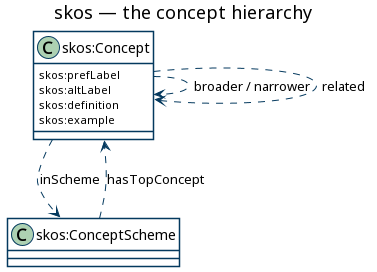
\includegraphics[width=\linewidth, height=0.6\textheight, keepaspectratio]{slides/im-101/skos/figs/skos.png}
    \end{column}
    \begin{column}{0.42\textwidth}
      \scriptsize
      \setlength{\itemsep}{0.5pt}
      \setlength{\parskip}{0pt}
      \textbf{Concepts}
      \begin{itemize}
        \item \texttt{skos:Concept} — a single idea in a vocabulary
        \item \texttt{skos:ConceptScheme} — the set that groups them
      \end{itemize}
      \vspace{0.4pt}
      \textbf{Relations (concept $\to$ concept)}
      \begin{itemize}
        \item \texttt{broader}\,$/\,$\texttt{narrower} — inverse hierarchy pair
        \item \texttt{related} — associative, non-hierarchical
        \item plus transitive variants (\ldots\texttt{Transitive})
      \end{itemize}
      \vspace{0.4pt}
      \textbf{Attributes \& membership}
      \begin{itemize}
        \item \texttt{prefLabel} / \texttt{altLabel} — display terms
        \item \texttt{definition} / \texttt{example} — meaning
        \item \texttt{inScheme} / \texttt{hasTopConcept}
      \end{itemize}
      \vspace{2pt}
      \begin{alertblock}{}
        A vocabulary is not an \emph{information model} — it is the \textbf{L0}
        layer: the named concepts we \emph{reuse} to describe L1.
      \end{alertblock}
    \end{column}
  \end{columns}
\end{frame}
